\documentclass[aps,prstper,reprint]{revtex4-1}
\usepackage{graphicx}
\usepackage{hyperref}
\hypersetup{colorlinks=true,urlcolor=blue,citecolor=blue,linkcolor=blue}
\urlstyle{same}

\newcommand\corinnesays[1]{\textcolor{red}{[\sc CAM: {\em#1}]}}
\newcommand\davidsays[1]{\textcolor{blue}{[\sc DR: {\em#1}]}}

\begin{document}

\title{Paradigms in Physics 2.0}
\author{David Roundy}
\email{roundyd@physics.oregonstate.edu}
\author{Elizabeth Gire}
\author{Ethan Minot}
\author{Emily van Zee}
\affiliation{Department of Physics, Oregon State University, Corvallis, Oregon, 97331}
\author{Corinne A. Manogue}
\affiliation{Department of Physics, Oregon State University, Corvallis, Oregon, 97331}

%\keywords{}

\maketitle

In 2016, the Department of Physics at Oregon State University began a
process to revise our Paradigms in Physics curriculum for physics
majors.  We began with a colloquium to inform the department of our
plans and request their assistance, followed by a
survey of students and faculty as well as individual interviews with
the faculty teaching each course.  As we developed a plan to
address student- and faculty-identified challenges in the curriculum,
we met with each faculty member individually to explain and refine our
proposal, which was unanimously approved by the faculty.  Major
changes include major changes to several courses (math
methods, computational physics, modern physics, electronics, and
classical mechanics), including the introduction of two sophomore-year
courses designed specifically to help prepare students for their
upper-division courses.

This paper will describe both the process of the reform and its
outcome, but the emphasis of the paper and the research aspect of it
will be on the process by which we developed the changes and arrived
at consensus.  This is paper is thus on the coarse-grained picture of
how one department acheived a broad-scale reform of its curriculum,
which we expect will serve as a valuable balance to the more
fine-grained view that is needed for classroom activities.  In
addition to the Paradigms 2.0 reform, we will briefly introduce the
original effort that began in 1996, and give a bit more detail on how
that reform was maintained and refined during the intervening decades.

This story of how we achieved a dramatic curriculum change will be
useful for other departments considering a reform of their curriculum.
Few departments embark on such an endeavor, and publishing a blueprint
for how we managed this will be helpful for others seeking to reform
their curriculum.

\paragraph*{Theoretical basis for the work}
The framework for this {\bf empirical study} was adapted from studies
of organizational decision-making\cite{beach2006leadership}.  Like the
process that led to Paradigms 1.0, the Paradigms 2.0 process is a
``shared vision'' type of change\cite{henderson2010}. Changes to the
course structures of the physics curriculum emerged from discussions
among the members of the department. The Paradigms~2.0 process began
in the Winter of 2016, after the faculty agreed to the process during
the previous year.

\paragraph*{Research questions}
\begin{itemize}
\item What was the culture of the department when the faculty initiated revising the upper-level physics curriculum? In
  particular, what were the participants' beliefs about teaching and
  learning?
\item What motivated making changes and how did the faculty form a
  coherent vision for the new program?
\item How did the faculty develop and communicate plans for this new
  curriculum?
\item How have they changed instruction based upon the proposals that
  the faculty approved with an unanimous vote?
\end{itemize}
\paragraph*{Research methods}
We performed interviews of faculty before, during and after the
Paradigms 2.0 process, gave surveys to students and faculty, and had
an observer take notes during all Paradigms 2.0 meetings.

%% The Paradigms in Physics project began in 1996, when three faculty
%% members at Oregon State applied to the NSF for funding to redesign the
%% upper-division curriculum.  The motivation for the original Paradigms~1.0
%% project was in fact similar to the motivation for Paradigms~2.0: a
%% desire to soften the ``brick wall'' encountered by students upon
%% reaching the junior year, within the constraint that transfer students
%% must be able to graduate with two years of upper-division
%% courses~\cite{manogue2001paradigms}.  On top of this, there was a
%% desire to provide students with a broad knowledge of physics prior to
%% the GRE exams in the fall of their senior year.  The process of
%% redesigning the curriculum was guided by the creation of index cards
%% listing subject content, and sorting these cards into courses.  This
%% process involved the entire faculty, and culminated in a unanimous
%% agreement to adopt the resulting curriculum.

%% The resulting curriculum was primarily composed of intensive junior-year \emph{Paradigm}
%% courses, followed by more conventional senior-year courses.
%% The \emph{Paradigm} courses meet every day for a total of seven
%% hours per week for 3 weeks.  These courses incorporate
%% laboratory experiences and active engagement into the class, and
%% typically have two problem sets per week.  These courses also had
%% integrated math content, and were followed by a \emph{Math Methods} course.
%% The senior-year courses are more traditional 3-credit courses which meet
%% three hours per week for an entire 10-week quarter.

%% Two decades have passed since the original Paradigms~1.0 effort.
%% During this time we have made a number of changes: e.g. a new
%% first \emph{Paradigm} course was introduced to soften the beginning of the
%% junior year, the order of courses was shuffled more than once, \emph{Math
%% Methods} was moved from the beginning of the senior year to the end of
%% the junior year, and a computational laboratory course was introduced
%% to accompany the junior-year \emph{Paradigm} courses.  The faculty maintained the tradition of meeting
%% every three weeks to discuss issues relating to upper-division
%% teaching.  New faculty arrived and learned to teach the new courses,
%% and introduced their own ideas to the courses.

%% %\subsection{Motivation for Paradigms 2.0}
%% A number of factors motivated us to embark on the
%% Paradigms~2.0 process.  In the last two decades, we have observed
%% a number of challenges students face in our major.  While in many cases we
%% addressed these by changing and reordering the courses, we felt a look
%% at the entire curriculum was in order.
%% In addition, our faculty
%% understanding of the details of the sequence was diminishing by attrition: 
%% while our younger
%% faculty are enthusiastic about the Paradigms program, many lack perspective on
%% where students are in a given course, and what content is essential
%% for students to grasp for a subsequent course.

%% \paragraph{Transfer students}
%% Our curriculum is strongly affected by our desire to accommodate
%% transfer students from community colleges.  This leads us to focus on
%% a physics major in which all upper-division courses are taken in two
%% years.  However, our current curriculum is very hard on students in
%% the fall of their junior year, and especially so for transfer
%% students.  So we aimed to structure and order the courses such that non-transfer
%% students could be better prepared for their junior year, while
%% transfer students could postpone a few courses so that the
%% Fall quarter of their junior year would be no more difficult than that of any other student.

%% \paragraph{Coupled curricular changes}
%% A backlog of curricular changes had accumulated that could not be
%% separated from an examination of the curriculum as a whole.  The requirements
%% for computational physics, the number of required electronics credits, and the
%% role of our modern physics course could not easily be addressed separately.

%% \paragraph{New faculty}
%% % Corinne, Henri, David McI, Janet, Tom = 5

%% % David R, Ethan, Oksana, Bo, Guenter, Weihong, Matt, Yun-Shik, Heidi,
%% % Liz, Davide = 11
%% Only 5 of our 16 current tenure-line faculty were involved in the
%% original Paradigms~1.0 effort.  Some of the newest faculty have only a
%% superficial understanding of our course structure.  This poses a
%% challenge when these professors teach courses that are closely
%% intertwined with one another.

%% \section{Paradigms 2.0 process}
%% Like the process that led to Paradigms 1.0, the Paradigms 2.0 process
%% is a ``shared vision'' type of change \cite{henderson2010}. Changes to
%% the course structures of the physics curriculum emerged from
%% discussions among the members of the department. We began the
%% Paradigms~2.0 process in the Winter of 2016, having in the previous
%% year obtained faculty agreement, and support from our Department head.
%% The process was spearheaded by a committee of four (the authors DR,
%% EG, EM, and CAM, with EvZ present at meetings documenting our
%% process).  During the Winter quarter, we informed the community of our
%% process through a colloquium, and collected student and faculty
%% perspectives on the existing curriculum.  We then interviewed faculty
%% who recently taught each of our existing courses to document topics
%% that were currently covered.  This resulted in a total of $\sim$700
%% index cards in $\sim$30 stacks, with each stack corresponding to one
%% course, and each card describing a topic, color-coded as in
%% Fig.~\ref{fig:schedule}.

%% The committee met twice a week to discuss existing challenges and sort
%% the cards into new stacks corresponding to new and reordered courses.
%% When we discussed major changes to a course, we often invited
%% interested faculty to join us to provide their own perspective on
%% possible challenges and improvements.  Once we had a draft proposal,
%% we began inviting each faculty member in to see the cards and discuss
%% the proposed sequence of courses.  In addition, we had a focus group with
%% all the current students to explain the proposed changes and request
%% feedback.

%% After incorporating the feedback from  individual meetings with every
%% faculty member, we scheduled
%% two full faculty meetings with a week in between.  In the first meeting,
%% we presented our proposal in detail and invited questions, but not discussion.
%% This was needed for a couple of reasons:  those faculty we met with first
%% may not have seen the final proposal, and some faculty during their
%% individual meetings chose to focus on a small subset of the
%% curriculum, often relating to courses they had themselves taught.
%% During the following week faculty engaged in hallway discussions of the proposal.
%% This week helped ensure that the faculty did not feel rushed into a vote.
%% In the second faculty meeting, we again presented our proposal, and opened
%% the floor for discussion.  After considerable discussion, largely on
%% changes that were not part of the proposal, the faculty unanimously voted to adopt
%% the proposed changes.

%% \begin{figure}
%% \includegraphics[width=\columnwidth]{vertical-schedule}
%% \caption{Hypothetical student schedule in the new curriculum.
%%   Transfer students begin in year 3, and take the marked additional
%%   courses.\label{fig:schedule}}
%% \end{figure}

\acknowledgments{This work was supported by the National Science
  Foundation under Grant No. 1323800 Supplement.}

% For a longer bibliography, delete the thebibliography block above, then comment in 
% these two lines to use a .bib file with BibTeX.
\bibliographystyle{apsrev}  	% supercedes the longbibliography option, so leave commented out if you want to display article titles
\bibliography{paper}  	% don't include the .bib suffix

\end{document}
